\subsection{Estad\'istica Descriptiva}
Obtener informaci\'on desde una muestra, que permita entender o formular hip\'otesis acerca del fen\'omeno que se estudia por medio de:\\
Gr\'aficos: descripciones cualitativas de una muestra.\\
Estadisticas: descripciones cuantitativas de tendencia y variable de una muestra.\\

\subsection{Medidas de Tendencia}

\subsubsection{Moda}
Valor o clases de valores que se observa con mayor frecuencia
\subsubsection{Media}
Centro geom\'etrico del conjunto de valores observados.
$\overline{x} = \frac{1}{n} \sum_{i=1}^n x_i$
\subsubsection{Mediana} Valor que divide al conjunto de valores ordenados, en dos mitades. Obtiene valores mas representativos que la media, ya que no es tan sensible a valores muy distintos al resto.

\subsubsection{Percentiles}
Valores $\textbf{ordenados}$ que acumulan una cierta frecuenta relativa. El i-\'esimo percentil es el \textbf{primer} valor que acumula al menos $\frac{i}{100}$.

\subsubsection{Cuartiles}
Cuartiles $Q_1$ $\ldots$ $Q_4$ corresponden a los percentiles $\frac{25}{100}$ $\ldots$ $\frac{100}{100}$

\subsection{Medidas de Tendencia Datos Agrupados}
Permite reducir efectos de ruido o errores. Se pesa un intervalo y su frecuencia, no la frecuencia de un s\'olo valor.

\subsubsection{Media Muestral}

$\overline{x} = \sum_{i=1}^k f_i C_i$\\
donde:\\ \\
$f_i$: $\textbf{Frecuencia relativa}$ de la clase.\\
$C_i$: Marca de clase: $\frac{maximo - minimo}{2}$

\subsubsection{Moda}
Clase con \textbf{mayor frecuencia}

Moda $= L + a_M(\frac{D_1}{D_1 + D_2})$\\
donde:\\ \\
L: Limite inferior clase modal\\
$a_M$: Amplitud Clase Modal\\
$D_1$: $n_M-n_1$\\
$D_2$: $n_M-n_2$\\
$n_M$: Frecuencia absoluta Clase Modal\\
$n_1$: Frecuencia absoluta clase anterior\\
$n_2$: Frecuencia absoluta clase posterior\\

\subsubsection{Mediana}

$M_e = L + a_e \frac{\frac{1}{2}-F_{e-1}}{f_e}$\\ \\

L: Limite inferior de Clase Mediana.\\
$F_{e-1}$: \textbf{Frecuencia Relativa Acumulada} hasta antes de Clase Mediana.\\
$f_e$: frecuencia Relativa Clase Mediana.\\
$a_e$: Amplitud Clase Mediana.\\

\subsubsection{Percentiles}

$P_i = L + a_{p_{i}} \frac{\frac{i}{100} - F_{p_i-1}}{f_{p_i}}$\\ \\
L: Limite inferior percentil i-esimo.\\
$F_{p_{i-1}}$: Frecuencia Relativa acumulada antes de la clase percentil i-esimo.\\
$a_{p_i}$: Amplitud percentil i-esimo.\\
$f_{p_i}$: Frecuencia Relativa de la clase del percentil i-esimo.\\

\subsubsection{Cuartiles}

$Q_i = L + a_{C_i} \frac{\frac{i}{4} - F_{C_i-1}}{f_{C_i}}$\\ \\
L: Limite inferior cuartil i-esimo.\\
$F_{p_{i-1}}$: Frecuencia Relativa acumulada hasta antes de la clase del cuartil i-esimo.\\
$a_{p_i}$: Amplitud cuartil i-esimo.\\
$f_{p_i}$: Frecuencia Relativa de la clase del cuartil i-esimo.\\

\subsection{Medidas de Dispersi\'on}

Grado de variabilidad con respecto a las tendencias.

\subsubsection{Indice de Variacion}
Frecuencia con que no se observa la moda o la c lase modal en la muestra.\\
$T = 1 - f_m$

\subsubsection{Varianza Muestral}
Promedio de las diferencias al cuadrado con respecto a la media.\\
Para datos no agrupados:\\
$s^2 = \frac{1}{n} \sum_{i=1}^n (x_i - \overline{x})^2$\\
Para datos agrupados:\\
$s^2 = \sum_{i=1}^n f_i(x_i - \overline{x})^2$\\ \ \ \ \ donde $f_i$: Frecuencia relativa de Clase i.

\subsubsection{Desviacion Estandar}
Tiene las mismas unidades de medida que las observaciones de la muestra.\\
Para datos no agrupados:\\
$s = \sqrt{\frac{1}{n} \sum_{i=1}^n (x_i - \overline{x})^2}$\\
Para datos agrupados:\\
$s = \sqrt{\sum_{i=1}^n (x_i - \overline{x})^2}$

\subsubsection{Desviacion Media}
Promedio de las diferencias absolutas con respecto a la media, tiene las mismas unidades de medida que las observaciones de la muestra.\\
Para datos no agrupados:\\
$MD = \frac{1}{n} \sum_{i=1}^n |x_i - \overline{x}|$\\
Para datos agrupados:\\
$MD = \sum_{i=1}^n f_i|x_i - \overline{x}|$

\subsubsection{Rango}
Dferencia entre el maximo y el minimo valor observado en la muestra.

\subsubsection{Rango Percentil}
Diferencia entre $P_{90}$ y $P_{10}$. Aproximacion mas robusta al rango.\\
$PR = P_{90} - P_{10}$

\subsubsection{Rango Intercuartilico}
Distancia promedio de los cuartiles con respecto a la mediana (segundo cuartil).\\
$IQR = \frac{Q_3 - Q_1}{2}$

\subsubsection{BoxPlots}

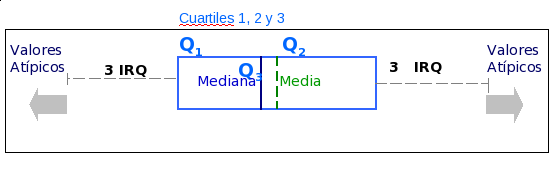
\includegraphics[scale=0.5]{images/boxplot}\\
\textbf{OJO:} el dibujo esta malo, Q1 esta al principio de la cajita, Q2 esta en la posicion de la mediana y Q3 esta al final de la caja.
Se entiende tambien que el IRQ de la izquierda es ``-3IRQ'' y no 3IRQ
Representacion visual para describir simultaneamente, varias caracteristicas importantes tales como:
\begin{itemize}
\item Centro
\item Dispersion
\item Asimetria de la distribucion
\item Identificar valores atipicos
\end{itemize}
